\documentclass[12pt]{report}

\usepackage{graphicx}

\begin{document}

\section*{Introduction}

The trained cGAN model provides a CHM inferred from the user sketch and the DEM. However, even though the CHM provides tree heights to within 1 meter accuracy, and at 0.9 meter per pixel resolution, the exact locations and species of individual trees that might produce such a CHM is unknown. The process of determining the species and locations of such trees, we will refer to as \textit{species assignment} and \textit{canopy placement}, respectively. In this section, we present an algorithm that performs canopy placement based on trees' competition for sunlight, as well as a method that performs species assignment based on a specified proportion of the CHM that each species represents.

\section*{Species assignment}

Before canopy placement is done, it is preferable to know the species of each individual tree. This is because the species of a tree tends to heavily affect the relationship between its height and crown radius, which in turn affects the competition for sunlight between trees.

The basic idea behind the species assignment method we present here, is that the user should have some intuitive input into the composition of species on the landscape. In previous work, a user would have set adaptability functions for each species. These functions dictate how a given species adapts to certain abiotic conditions, such as water, sunlight, temperature and slope. However, it can be very difficult to know how a given setting of these functions would affect the composition of species on a given landscape. 

The algorithm we present here takes as input a percentage of the CHM covered by each species, and optionally, a constraint on the adaptability of any species to the abiotic conditions. For example, a user may give as specification that 70\% of the CHM must consist of species 1, while 30\% consists of species 2, where species 1 is restricted to conditions of high soil moisture. After inputs have been given, the algorithm finds a set of suitability functions for each species that results in a composition that satisfies the user's specification and constraints within some margin of error.

Each species has a suitability function for each abiotic condition, since it must adapt to each of the given abiotic conditions. In our case, we apply it to four: temperature, sunlight, soil moisture and slope. The number of suitability functions that must be found in order to satisfy the user's specification is therefore $4N_s$, where $N_s$ is the number of (\textbf{CANOPY}) species on the landscape.

Each species' suitability function is in the form of a Gaussian function. We use

\begin{equation}
f(x) = exp(\frac{(x - c)^{4.5}}{w^{4.5}} ln(a))
\label{equation:adaptFunction}
\end{equation}


where $f(x)$ is the plant's adaptability value if the abiotic condition has a value of $x$, $c$ is the value of the abiotic condition at which the plant has an optimal adaptation, and $w$ and $a$ describe the hardiness of the plant. In particular, $w$ is how much the value of the abiotic condition must differ from $c$ for the plant to reach an adaptability value of $a$ or lower. In the graphic below, $a = 0.1$, but we use $a = 0.01$ in our pipeline.

Graphically, $f(x)$ has the following form

\begin{center}
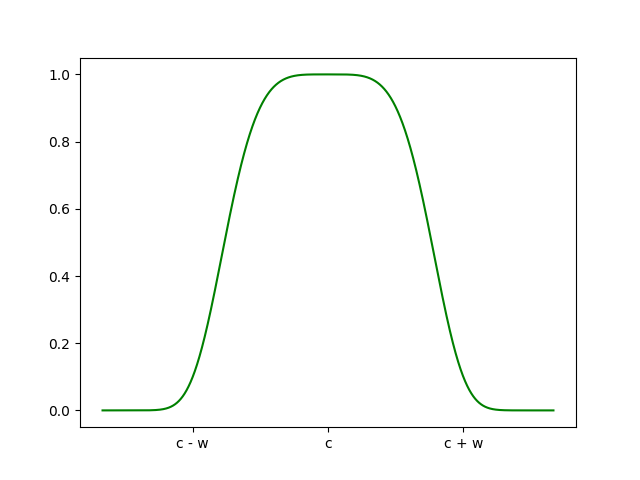
\includegraphics[scale=0.7]{singleGauss}
\end{center}

As implied by $f(x)$, the adaptability value of a species for a given abiotic condition ranges between 0 and 1, where 0 is the worst adaptation and 1 is an optimal adaptation.

To determine which species must get assigned to a given pixel, we compute which plant species will be most likely to survive on that location. To achieve this, $f(x)$ is computed for each species, then again for each abiotic condition. We use the same reasoning as used in (GAIN2017), where the worst adaptation out of all abiotic conditions determines a tree's final adaptation to its conditions. Therefore, we take the minimum of all a species' adaptability values for a given pixel as its final adaptability value for that pixel. Once all pixels have been assigned species, we count the number of pixels that each species has been assigned to and divide by the number of pixels in the CHM. This results in a measure of how close the current adaptability functions resemble what is required by the user's specification. 

The way in which the adaptability functions for each species are modified, is via the parameters $c$ and $w$ in equation~\ref{equation:adaptFunction}. Observe that 

\[
\frac{\partial f(x)}{\partial w} = -4.5 \frac{(x - c)^{4.5}}{w^{5.5}} ln(a) f(x) \geq 0
\]

Therefore, increasing $w$ for a given plant's adaptation function (that is, increasing its hardiness) causes its adaptation function to increase where $x \neq c$. When a plant's percentage representation with its current parameters is below its required representation, we increase its hardiness for all abiotic conditions. 

\end{document}